\chapter{Identyfikacja}


\section{Model obiektu}

Obiektem sterowania był model Strejca opisany  transmitancją:
\begin{equation}\label{key}
G(s) = \dfrac{K_0}{(T_0 \cdot s + 1)^n} \cdot e^{-\tau \cdot s} 
\end{equation}
Na potrzeby niniejszej pracy ograniczono się do obserwacji zachowania modeli rzędu pierwszego, drugiego oraz trzeciego.
 
 
\section{Optymalizacja nastaw regulatora}

Do optymalizacji nastaw regulatorów wykorzystana została funkcja \textit{fmincon} z pakietu MATALB. Badania przeprowadzone zostały dla jednego zestawu parametrów z jednoczesną zmianą rzędu obiektu, którym sterowano.

\subsection{Zestawy parametrów}

W tabeli \ref{tab_par} zamieszczono przyjęte wartości parametrów.
\begin{table}[]
	\centering
	\caption{Zestawy parametrów dla których przeprowadzano optymalizację nastaw regulatorów.}
	\label{tab_par}
	\begin{tabular}{|c|c|} \hline
	Parametr & Wartość \\ \hline
	$K_{w1}$                                             & 10 \\ \hline
	$K_{w2}$                                                                                         & 5 \\ \hline
		$T_{w2}$                                                                                          & 0.1 \\ \hline
		$T_0$                                                                                             & 1 \\ \hline
		$K_0$                                                                                             & 10 \\ \hline
		$\tau$                                                                                            & 1 \\ \hline
	\end{tabular}
\end{table}


\subsection{Optymalizacja nastaw regulatorów}
Dla kolejnych zestawów parametrów opisujących system przeprowadzano procedurę optymalizacji nastaw regulatorów minimalizując wska\'znik jakości opisany zależnością \ref{wsk_jak}. Proces optymalizacji przeprowadzany był dla różnych wartości zadanych w obecności znanego zakłócenia $z_2$ (zakłócenie skokowo zmieniające swoją wartość) oraz nieznanego zakłócenia $z_1$. Przebiegi owych zakłóceń przedstawiono na rysunku \ref{fig_zaklocenia}. 

\begin{figure}[h!]
	\centering
	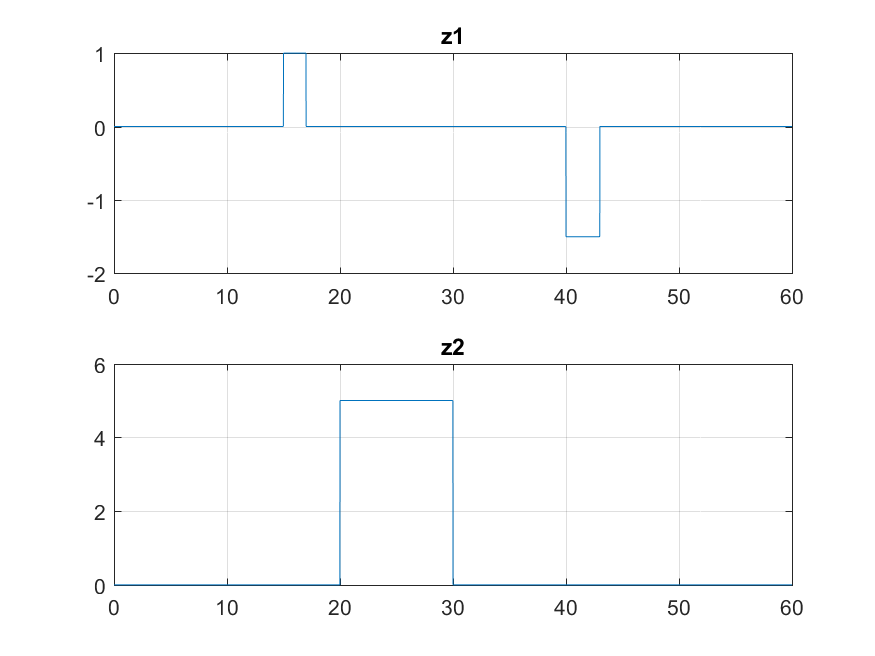
\includegraphics[scale = 0.7]{fig/Z1_New_Signal_1/fig3_1_5.png}
	\caption		
	{Zakłócenia.}
	\label{fig_zaklocenia}
\end{figure} 

Dla przedstawionych powyżej przebiegów zakłóceń przeprowadzono optymalizację a otrzymane nastawy dla poszczególnych obiektów zamieszczono w tabelach \ref{par_reg_zes1} - \ref{par_reg_zes3}. 

\begin{table}[h!]
	\centering
	\caption{Parametry regulatorów dla obiektu pierwszego rzędu.}
	\label{par_reg_zes1}
	\begin{tabular}{|c|c|c|c|c|c|c|c|}
		\hline
		\multicolumn{1}{|l|}{\begin{tabular}[c]{@{}l@{}}Parametr regulatora\textbackslash\\ Wart. zadana\end{tabular}} & $P1$ & $D1$ & $P2$ & $D2$ & $P3$ & $I3$ & $Kr$ \\ \hline
		5 & 0,0210 & 0,0375 & 0,2631 & 3051,8095 & 0,0690 & 0,0495 & 0,5446  \\ \hline
		10 & 0,0136 & 0,0025 & 0,8315 & 0,5000 & 0,0011 & 0,0139 & 0,8967 \\ \hline
		20 & 0,1184 & 65,7395 & 0,1422 & 119,0489 & 0,0503 & 0,0000 & 0,1098 \\ \hline
		50 & 0,0800 & 2,3514 & 0,3671 & 537,5907 & 0,0402 & 0,0194 & 0,5373 \\ \hline
		70 & 0,0571 & 8,2291 & 0,2161 & 99999,4370 & 0,0489 & 0,0347 & 0,5372 \\ \hline
	\end{tabular}
\end{table}

\begin{table}[h!]
	\centering
	\caption{Parametry regulatorów dla obiektu drugiego rzędu.}
	\label{par_reg_zes2}
	\begin{tabular}{|c|c|c|c|c|c|c|c|}
		\hline
		\multicolumn{1}{|l|}{\begin{tabular}[c]{@{}l@{}}Parametr regulatora\textbackslash\\ Wart. zadana\end{tabular}} & $P1$ & $D1$ & $P2$ & $D2$ & $P3$ & $I3$ & $Kr$ \\ \hline
		5 & 0,747 & 0,000 & 1,317 & 0,917 & 0,017 & 0,010 & 1,203 \\ \hline
		10 & 0,091 & 0,038 & 1,046 & 352,383 & 0,086 & 0,000 & 1,098 \\ \hline
		20 & 0,103 & 0,986 & 0,515	 & 5,071 & 0,036 & 0,000 & 0,539 \\ \hline
		50 & 0,000 & 123,529 & 0,002 & 112,641 & 0,496 & 0,175 & 0,005 \\ \hline
		70 & 0,057 & 20,823 & 0,289 & 0,000 & 0,054 & 0,018 & 0,648 \\ \hline
	\end{tabular}
\end{table}

\begin{table}[h!]
	\centering
	\caption{Parametry regulatorów dla obiektu trzeciego rzędu.}
	\label{par_reg_zes3}
	\begin{tabular}{|c|c|c|c|c|c|c|c|}
		\hline
		\multicolumn{1}{|l|}{\begin{tabular}[c]{@{}l@{}}Parametr regulatora\textbackslash\\ Wart. zadana\end{tabular}} & $P1$ & $D1$ & $P2$ & $D2$ & $P3$ & $I3$ & $Kr$ \\ \hline
		5 & 0,101 & 1,082 & 0,445 & 0,329 & 0,044 & 0,000 & 0,541 \\ \hline
		10 & 0,103 & 0,085 & 0,607 & 0,450 & 0,093 & 0,009 & 1,222 \\ \hline
		20 & 0,103 & 3,252 & 0,460 & 123,929 & 0,028 & 0,000 & 0,544 \\ \hline
		50 & 0,016 & 3,921 & 0,007 & 6447,659 & 0,427 & 0,132 & 0,004  \\ \hline
		70 & 0,057 & 0,757 & 0,164 & 7,857 & 0,053 & 0,014 & 0,547 \\ \hline
	\end{tabular}
\end{table}

W tabeli \ref{wsk_jakosci_tab} przedstawiono wartości wskaźnika jakości dla wszystkich przeprowadzonych symulacji.

\begin{table}[h!]
	\centering
	\caption{Wartości wska\'znika jakości dla różnych wartości zadanych i różnych zestawów parametrów opisujących system.}
	\label{wsk_jakosci_tab}
	\begin{tabular}{|c|c|c|c|}
		\hline
		\multicolumn{1}{|l|}{\begin{tabular}[c]{@{}l@{}}Nr zestawu\textbackslash\\ Wart. zadana\end{tabular}} & 1 & 2 & 3 \\ \hline
		5                                                                                                     & 68,7359 & 47,761466 & 57,1911 \\ \hline
		10                                                                                                    & 120,7282 & 54,657476 & 75,8104 \\ \hline
		20                                                                                                    & 106,0193 & 73,950359 & 100,7350 \\ \hline
		50                                                                                                    
& 190,4820 & 203,0570 & 297,3518 \\ \hline
		70                                                                                                    & 262,3173 & 414,4438 & 525,3915 \\ \hline
	\end{tabular}
\end{table}

Na rysunkach \ref{wykres_1} - \ref{wykres_4} przedstawiono przykładowe przebiegi zawierające odpowiedzi obiektów dla różnych wartości zadanych.

\begin{figure}[]
	\centering
	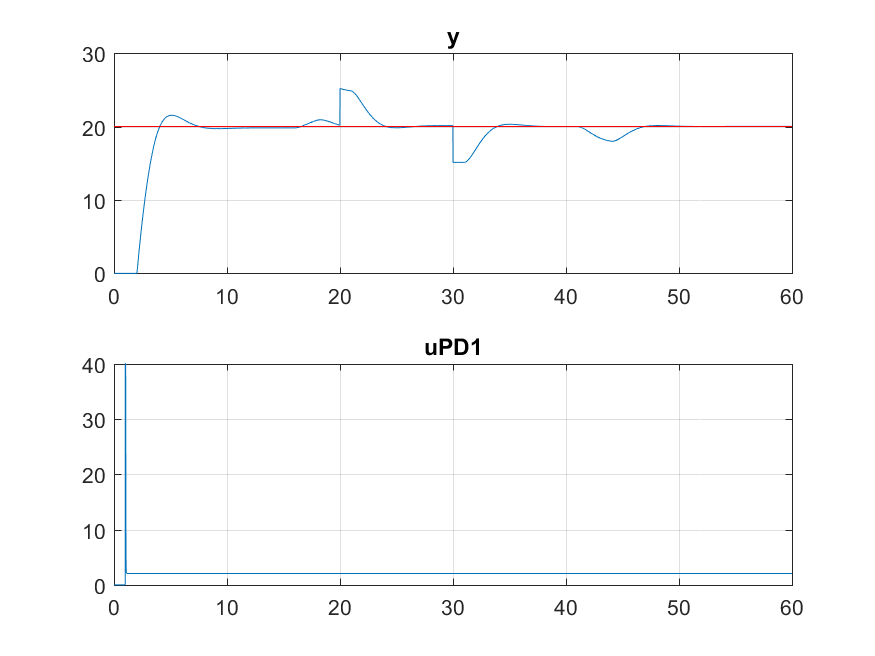
\includegraphics[scale = 0.7]{fig/Z1_New_Signal_1/fig1_2_20.png}
	\caption		
	{Odpowiedź obiektu drugiego rzędu, r = 20}
	\label{wykres_1}
\end{figure} 

\begin{figure}[]
	\centering
	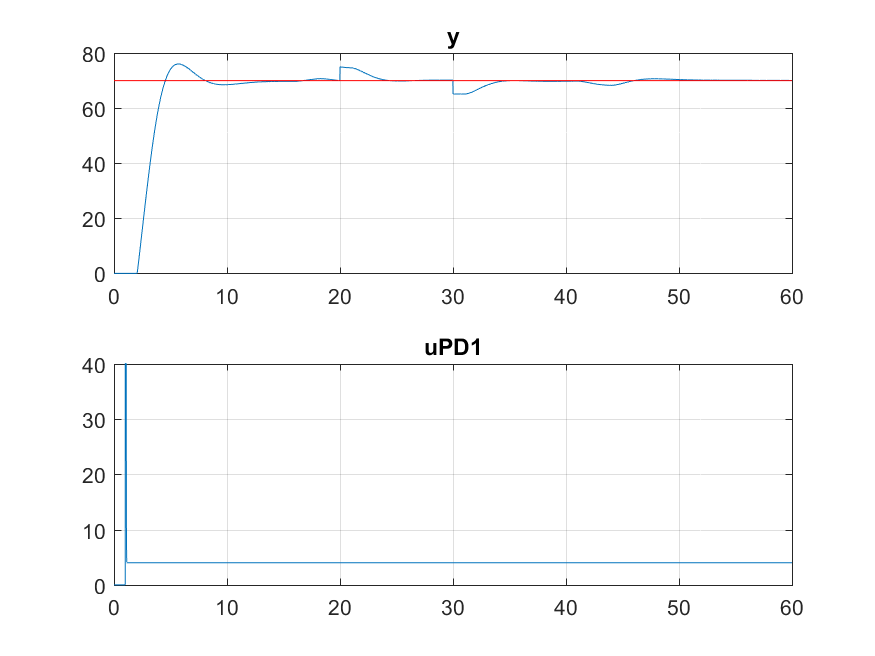
\includegraphics[scale = 0.7]{fig/Z1_New_Signal_1/fig1_2_70.png}
	\caption		
	{Odpowiedź obiektu drugiego rzędu, r = 70}
	\label{wykres_2}
\end{figure} 

\begin{figure}[]
	\centering
	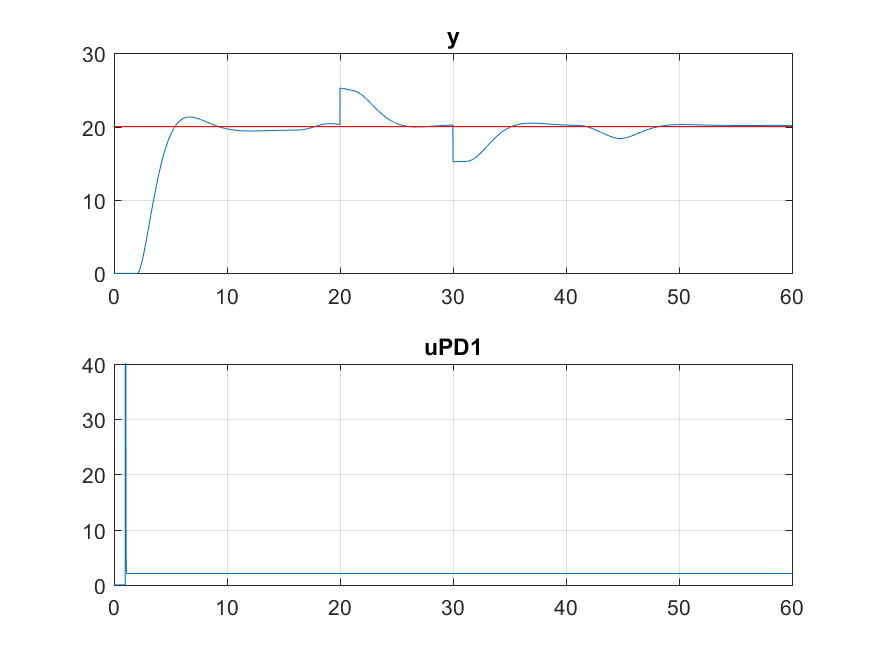
\includegraphics[scale = 0.7]{fig/Z1_New_Signal_1/fig1_3_20.png}
	\caption		
	{Odpowiedź obiektu trzeciego rzędu, r = 20}
	\label{wykres_3}
\end{figure} 

\begin{figure}[]
	\centering
	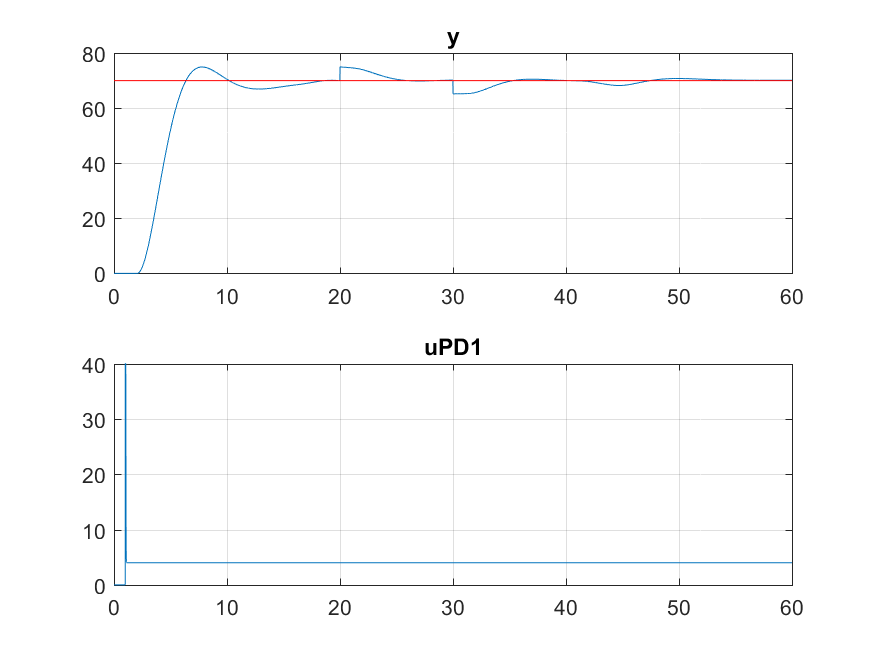
\includegraphics[scale = 0.7]{fig/Z1_New_Signal_1/fig1_3_70.png}
	\caption		
	{Odpowiedź obiektu trzeciego rzędu, r = 70}
	\label{wykres_4}
\end{figure} 